\documentclass[12pt]{article}
\usepackage[utf8]{inputenc}

\newenvironment{sol}[1][Solution]{\begin{trivlist}\item[\hskip\labelsep {\bfseries #1:}]}{\end{trivlist}}
\usepackage[margin=1in]{geometry} 
\usepackage{amsmath,amsthm,amssymb}
\usepackage{minted}
\usemintedstyle{vs}
\usepackage{graphicx}
\graphicspath{{./images}}
\usepackage{ amssymb }
\usepackage{times,url}  
\usepackage{hyperref}

\title{CS7381 Project 4 \\ 
Verilog Code Development using Cadence Xcelium }

\author{
Name: Bingying Liang \\
ID: 48999397\\  
Distance}
\date{March 26 2023}

\begin{document}

\maketitle

In previous projects, we learned how to use the MARS tool to develop and simulate MIPS assembly code.  Next, we will use the Verilog HDL (Hardware Description Language) to develop and simulate various MIPS components. 

We will use the Cadence Xcelium tool on the Lyle Unix servers.  Please go to my web site \href{http://lyle.smu.edu/~manikas/CAD_tool_info.html}{Links} to an external site. for information on how to do the following steps:
\begin{enumerate}
    \item Obtain a Lyle Unix account, if you do not already have one: \href{https://www.smu.edu/OIT/Services/genuse} {Links} to an external site.
    \begin{sol}
        \hspace*{\fill} \\
        \begin{center}
        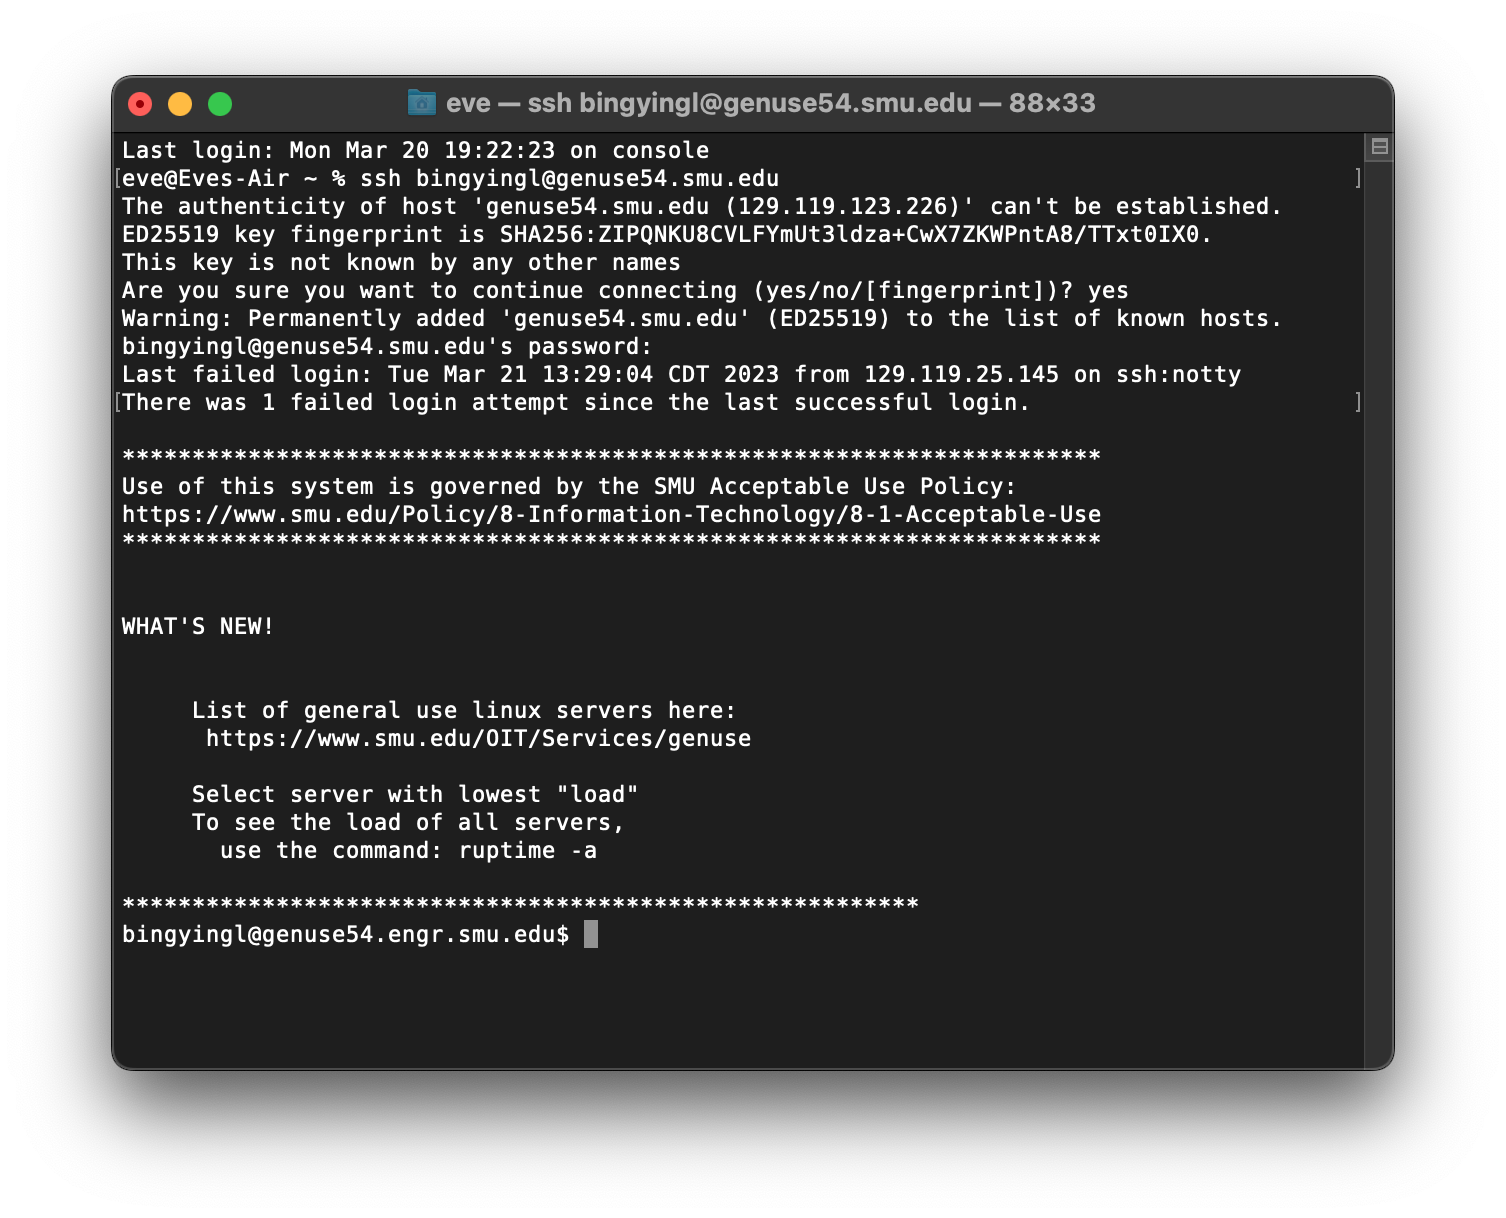
\includegraphics[width=0.8\textwidth]{1.png} 
    \end{center}
    \end{sol}
    \item Set up an X-Windows emulator on your computer.
    \begin{sol}
        I use XQuartz. And for OS, have to modify sshd\_config.
        \begin{center}
        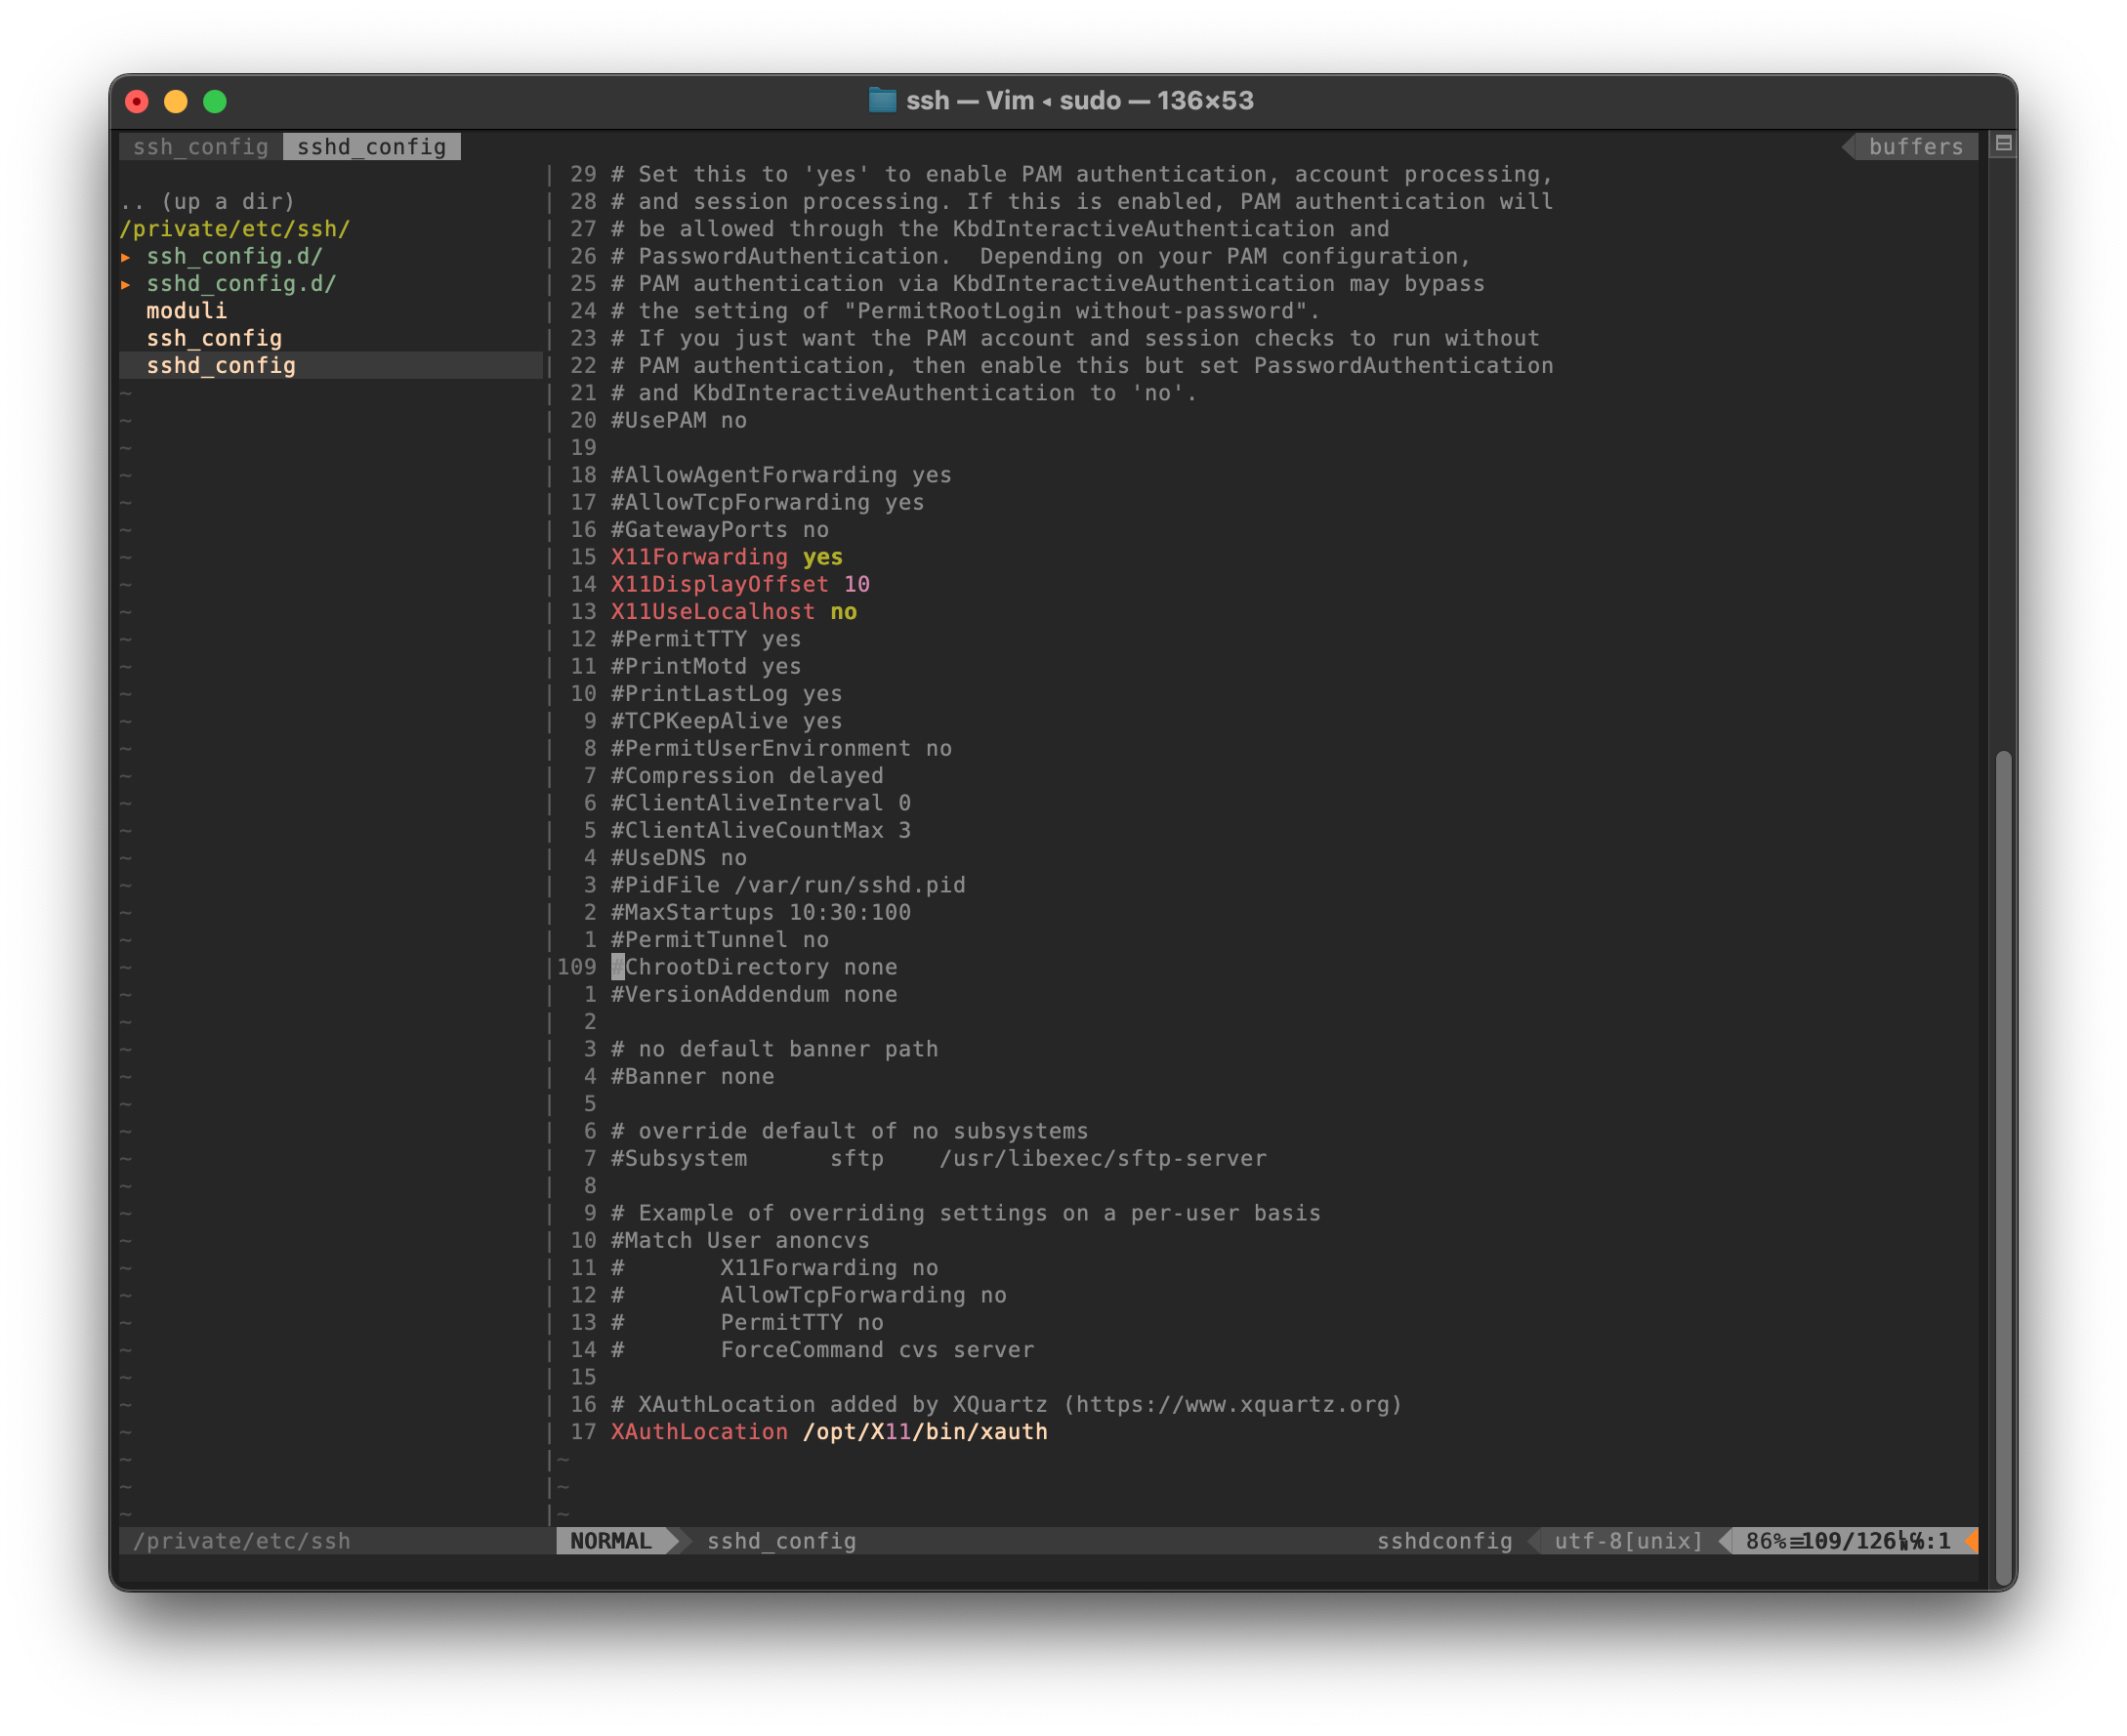
\includegraphics[width=0.9\textwidth]{2.png}
        
\includegraphics[width=0.9\textwidth]{3.png}
        \end{center}
    \end{sol}

\end{enumerate}
    After you have set up your computer to run Xcelium, do the following to complete the project:
    \begin{enumerate}
        \item Please download the following Verilog files:
        \begin{itemize}
            \item \href{https://smu.instructure.com/courses/106177/files/7251184?wrap=1}{S23\_MIPS\_ALU\_basic.v} - a Verilog module for a simple MIPS arithmetic/logic unit (ALU).
            \item \href{https://smu.instructure.com/courses/106177/files/7251189?wrap=1}{S23\_MIPS\_ALU\_basic\_tb.v} - the testbench for testing the ALU
        \end{itemize}
        \item This ALU performs the following 2 functions:
        \begin{itemize}
            \item Function code 1 to implement bitwise OR (A or B)
            \item Function code 7: set if $A < B$
        \end{itemize}
        \item Run the Verilog code using Xcelium:
        \begin{itemize}
            \item Use the command: \textbf{xmverilog S23\_MIPS\_ALU\_basic.v S23\_MIPS\_ALU\_basic\_tb.v}
            \item Note that a copy of the testbench output will be stored in the log file by Xcelium
            \item Please submit the resulting log file, edited with your name in the file.
        \end{itemize}
    \end{enumerate}
    \begin{sol}
    Upload File to the Server, and run the Verilog code. 
    \begin{center}
        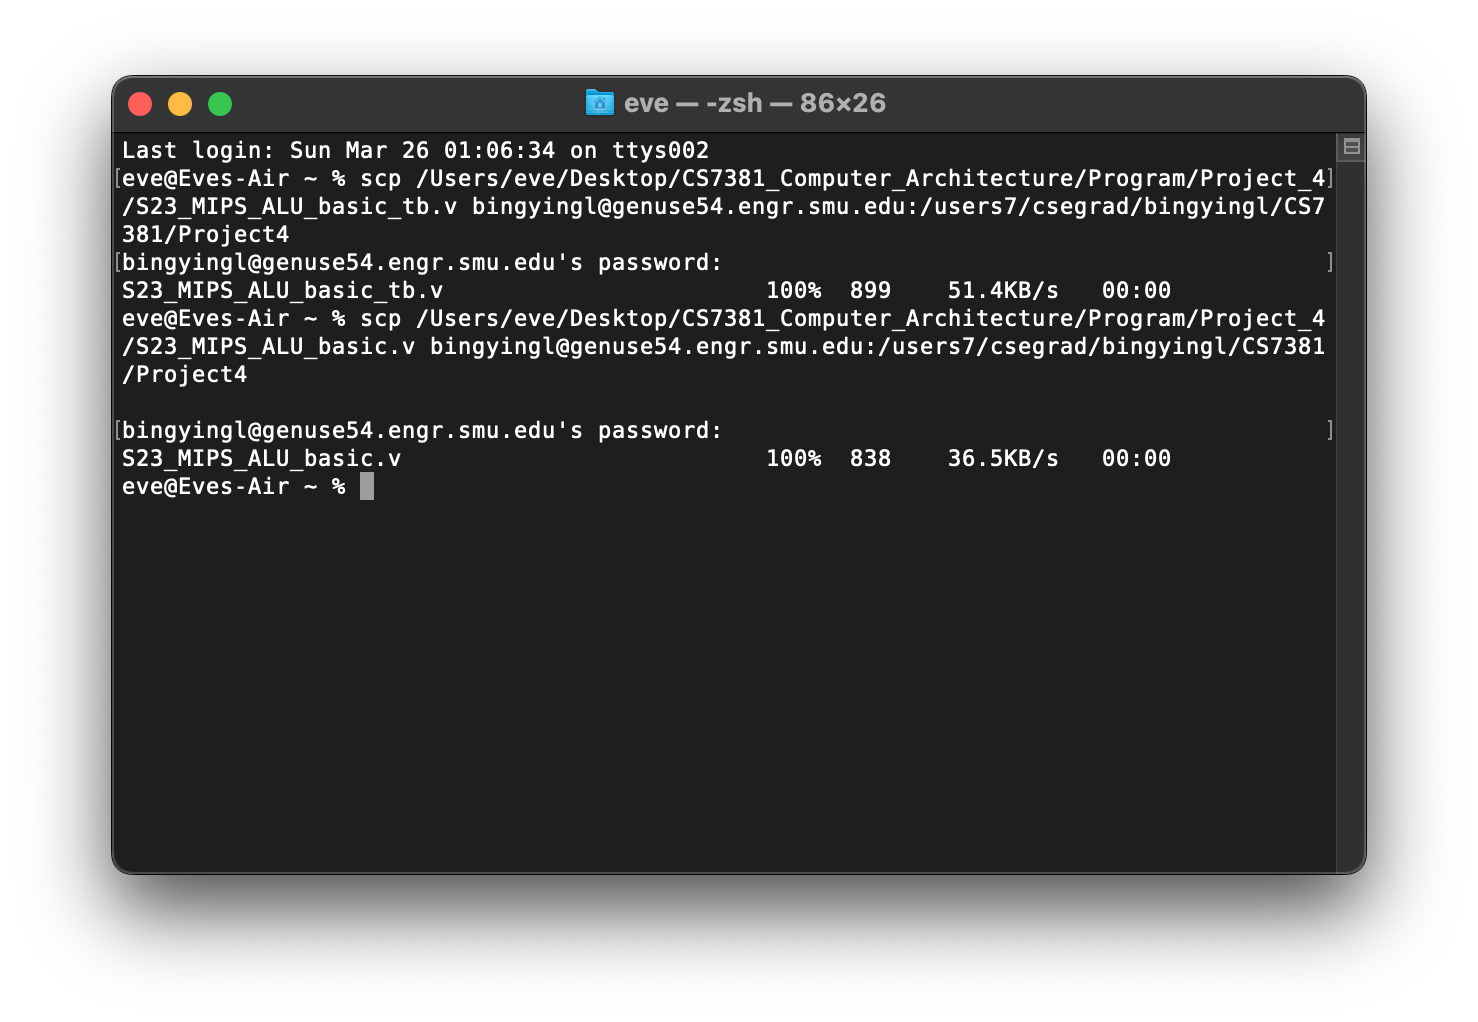
\includegraphics[width=0.9\textwidth]{4.png}
        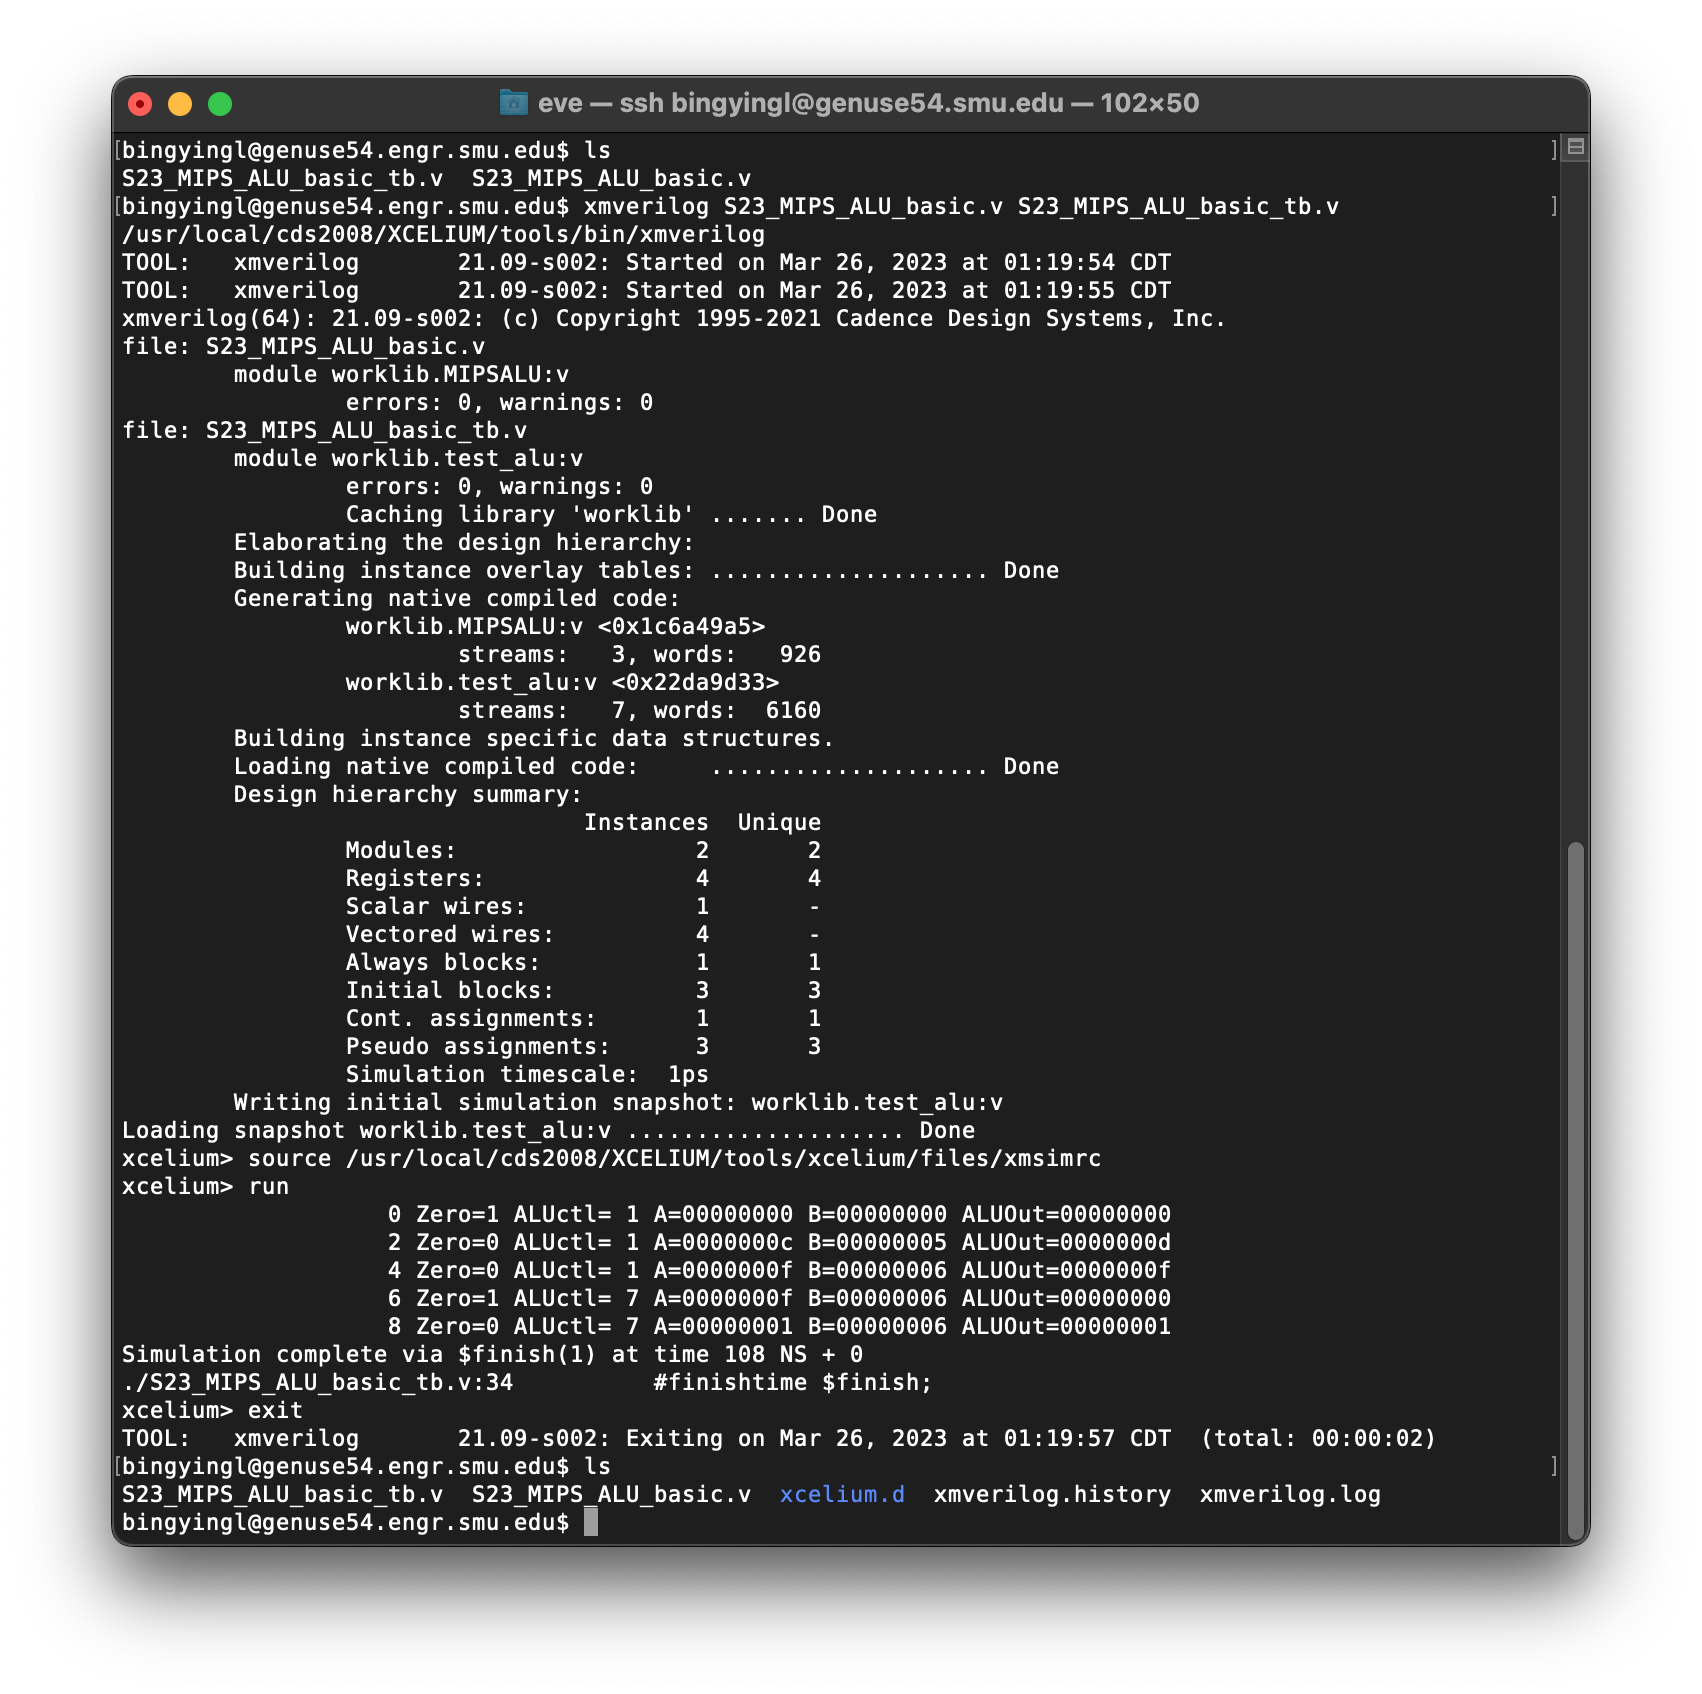
\includegraphics[width=0.9\textwidth]{5.png}
    \end{center}
    And then download the log file from the server
    \begin{center}
        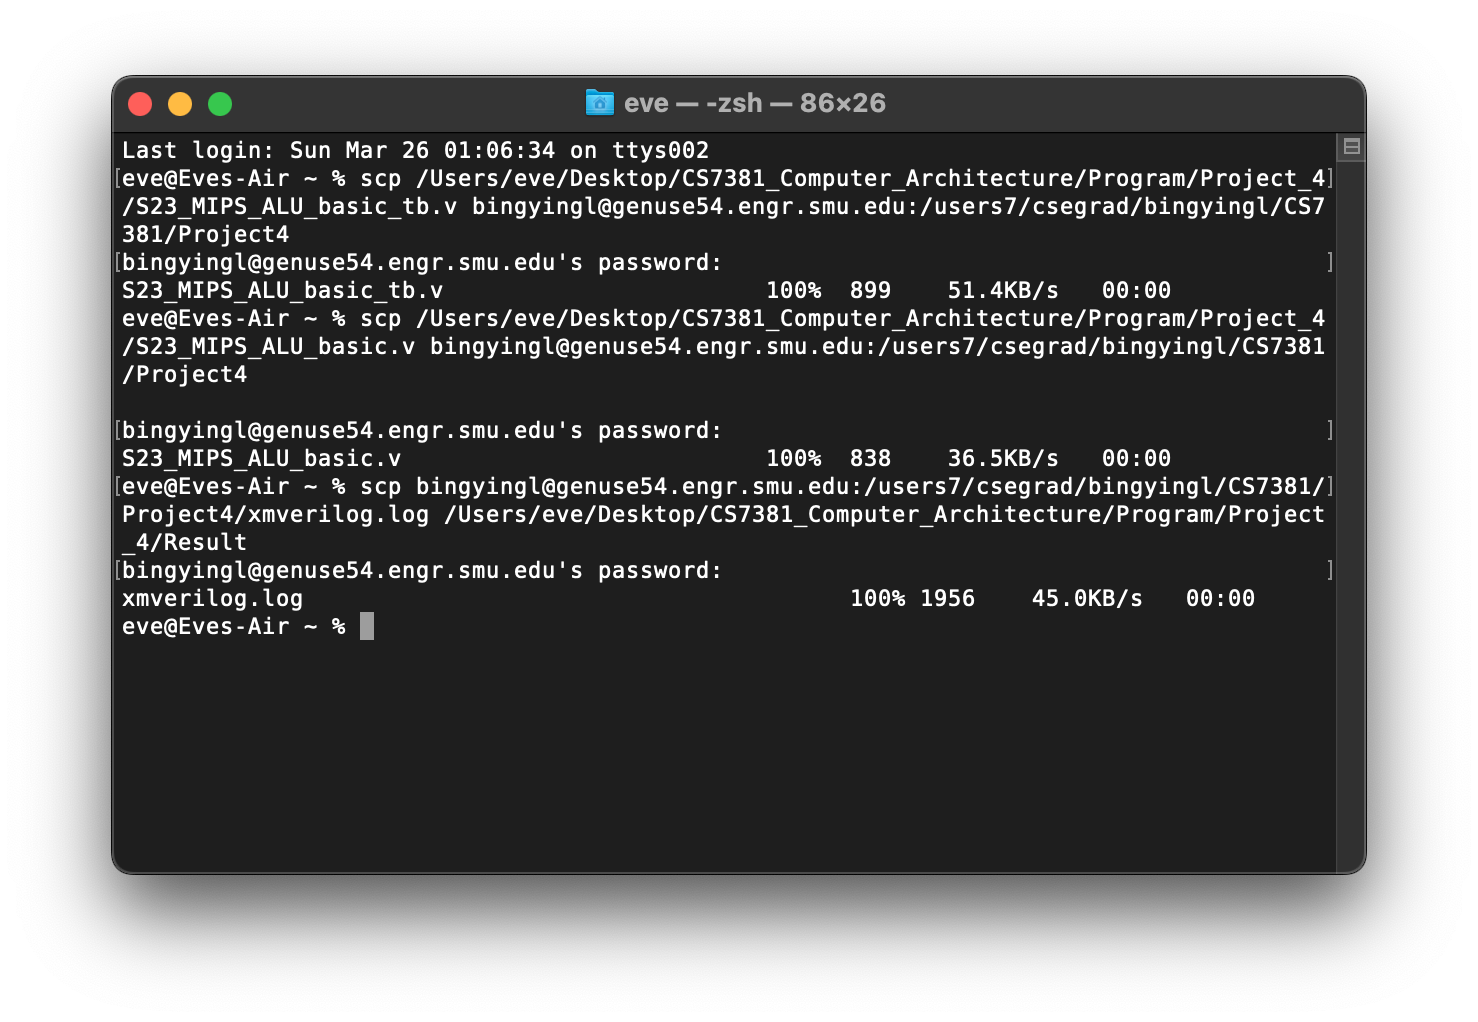
\includegraphics[width=0.9\textwidth]{6.png}
        
\includegraphics[width=0.9\textwidth]{7.png}
    \end{center}
    \end{sol}
\end{document}
